\documentclass[a4paper,11pt]{article}
\usepackage{graphicx}
\usepackage{hyperref}

\begin{document}
\begin{center}

\Huge\textbf{Functional Requirements\\}
																											
\vspace{2 cm}

\LARGE\textbf{Group Name:} Group 6\_b\newline
 
\vspace{0.5 cm}
\begin{tabular}{lr}
Jessica (JI) Lessev&13049136\\
Thabang (TM) Letageng&13057937\\
Michelle Swanepoel&13066294\\
Prenolan Govender&13102380\\
Fako (FJA) Peleha&12230830\\
Lutfiyya Razak&10198408\\
Ephiphania Munava&10624610\\
Maria Qumalo&29461775\\
\end{tabular}

\vspace{1cm}
\textbf{Git repository link:\\}
\url{https://github.com/u12230830/COS301\_6b}

\vspace{1cm}
\textbf{Date:} 27 February 2015
\end{center}




\newpage

%Section Functional requirements
\begin{center}
\huge\section{Functional Requirements}
\end{center}

\subsection{Use case prioritization}
Jessica and Michelle\\
\textbf{Critical}: CRUD Posts.\\
\textbf{Critical}: CRUD BuzzSpace.\\
\textbf{Critical}: Login.
\\
\\
Jimmy\\
\textbf{Critical}: Closing threads is very essential in maintaining order within the system. If a final answer to any query has been reached then there should be no further discussion regarding it. Alternatively, a request can be sent to the administrator to reopen the thread should there be any further developments with regard to the given problem.
\textbf{Critical}: The Hiding of Threads is also very essential to the integrity of the system. This allows the administrator to use their own discretion with regard to the given thread. If the content of the thread is misleading, vulgar, plagiarized etc. it is up to the administrator to see to it that the thread is blocked or hidden from other users to avoid any conflict.
\\
\textbf{Important}: The moving of content within the system is very important. It may occur that a similar issue has been raised in another thread or Buzz space. To avoid duplication of discussions, it is necessary do duplicate the solution. Another case exists where a post is not relevant to an active discussion but is very valuable to another. The administrator should therefore be able to actively move that content to a relevant Buzz space/thread.
\\
\textbf{Nict-To-Have}: It is preferable to summarize a thread i.e. to show only the root and the final answer and the social tags when entering a Buzz space. This makes for a finer design which is more organized and relieves the user of the trouble to rummage through tedious comment. Such a scenario would exist when the amount of content is hefty or when a discussion is lengthy. However, the system will not lose any significant value is this feature is omitted. In many systems, users have the option to expand or collapse threads.
\\
Ephi\\
\textbf{Critical}: Management of user profiles.
\\
\\
Thabang\\
\\
Prenolan\\
\textbf{Important}: Voting on and evaluation of posts.
\\
\textbf{Nice-To-Have}: Marking a post as the best answer.
\\
\\
Lutfiyya\\
\textbf{Important}: Evaluation Report
\\
\\
Maria\\


\subsection{Use case/ Services contracts}
Jessica and Michelle\\
\subsubsection{CRUD BuzzSpace}
\textbf{Pre-Condition:} User who want to create the BuzzSpace must be registered (if for a specific module, user must be registered for that module too) and logged in.
User must have the necessary permissions to create, update and delete a BuzzSpace.
No BuzzSpace with the same name may be created.
\\
\textbf{Post-Condition:} BuzzSpace will be archived for future reference.
\\
\textbf{Request and Results Data Structure:}
\\
\\
\subsubsection{CRUD Posts}
\textbf{Pre-Condition:} The user must be registered to the BuzzSpace to which he/she wants to CRUD a post.
The user must be logged in (except with read – will use “Guest user”).
To update and delete other users’ posts, the user should have certain permissions before it can be done.
User must adhere to length restriction on a certain level.
User must have a high enough status to post on a certain level.
\\
\textbf{Post-Condition:}If a post is read, it will be displayed as a read post.
If a post is updated, everyone who has read that certain post before, will be notified, and also the creator of the thread (even if he has not read it).
If a post is deleted, the creator of the thread will be notified.
After posting the user’s status should be changed according to the post.
If plagiarism is detected, notify the creator of the thread and BuzzSpace so that they can decide what to do (delete or update that post).
\\
\textbf{Request and Results Data Structure:}
\\
\\

\subsubsection{Login}
\textbf{Pre-Condition:} User must be registered.
\\
\textbf{Post-Condition:} User is now able to create, update and delete posts(his/her own) and have access to other functionality features.
\\
\textbf{Request and Results Data Structure:}
\\
\\

Jimmy\\
<<<<<<< HEAD

=======
\subsection{Summarizing threads}
\textbf{Pre-Condition}: The thread has exist.
\textbf{Pre-Condition}: The thread has to be closed. A conclusion was reached.
\\
\textbf{Post-Condition}: Only the root thread, social tags and the solution thread should be visible to the user. A link to the fully expanded thread and children should be available.
\textbf{Post-Condition}: The thread must still exist.
\\
\subsection{Hiding Threads}
\textbf{Pre-Condition}: The thread must exist.
\textbf{Pre-Contition}: The thread�s integrity has to questionable.
\\
\textbf{Post-Condition}: The thread must still exist.
\textbf{Post-Condition}: The thread must be hidden from the end users but visible to the system.
\\
\subsection{Closing threads}
\textbf{Pre-Condition}: The thread must exist.
\textbf{Pre-Contition}: A conclusion has to have been agreed upon.
\\
\textbf{Post-Condition}: The thread must still exist.
\textbf{Post-Condition}: No further sub-threads may be created. 
\textbf{Post-Condition}: Thread must be available for summary.
\\
\subsection{Moving Threads}
\textbf{Pre-Condition}: The thread must exist.
\textbf{Pre-Contition}: The destination has to relevant to the thread.
\\
\textbf{Post-Condition}: The thread must still exist.
\textbf{Post-Condition}: The thread may or may not exist depending on the relevance to the space.
>>>>>>> origin/master
Ephi\\
\subsubsection{Managing User Profile}
\textbf{Pre-Condition}: A user must be a registered member of the university and a registered member of one or more modules available on the BuzzSpace.
\\
\textbf{Post-Condition}: The user is registed and can now login thus it is now possible for the user to comment, tag and vote for threads on the BuzzSpace. The user now has a profile on the BuzzSpce meaning the can have a status, thus enabling diffent functionality at different status levels.
\\
\\
<<<<<<< HEAD
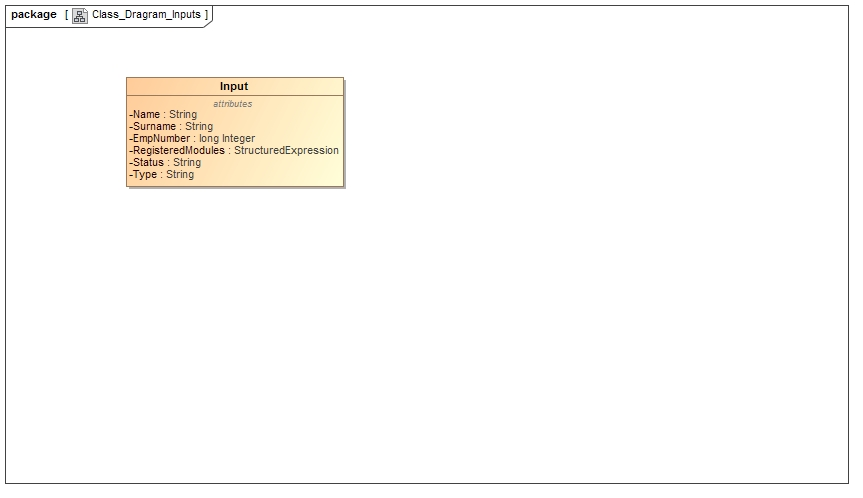
\includegraphics{Images/ManageUserProfile/Class_Dragram_Inputs}
=======
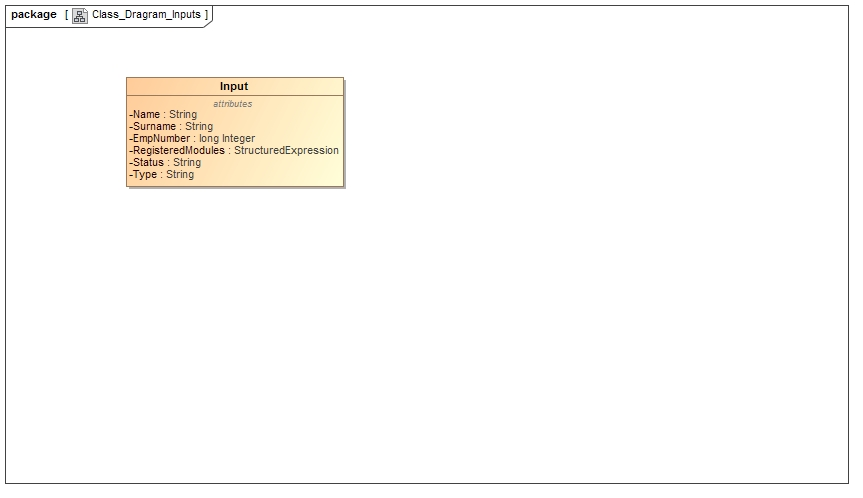
\includegraphics{Images/ManageUserProfile/Class_Diagram_Inputs}
>>>>>>> origin/master
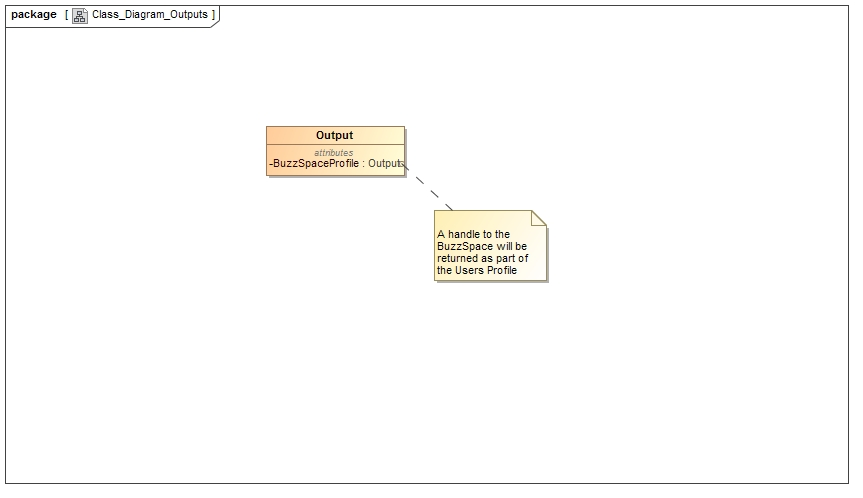
\includegraphics{Images/ManageUserProfile/Class_Diagram_Outputs}
\\

Thabang\\
\subsubsection{Filtering}
\textbf{Description:}This module provides a search and filter functionality. Users can filter the Buzz Space by tags, date,user or by user-rating. They can also search through the Buzz Space by entering a search-phrase in a search box, alternatively they can both search and filter i.e filter the search-results by tags, date, user or user-rating. 
\\
<<<<<<< HEAD
\textbf{Pre-Condition:} A specific Buzz Space has to have been created for a user to be able to search and/or filter.
\\
\textbf{Post-Condition:} Upon clicking the submit button, the search and/or filter results will be automatically displayed for the user to see.
\\
\\
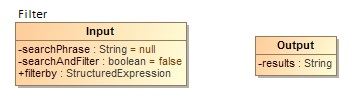
\includegraphics{Images/SearchAndFilter/Filter_input_output}
\\
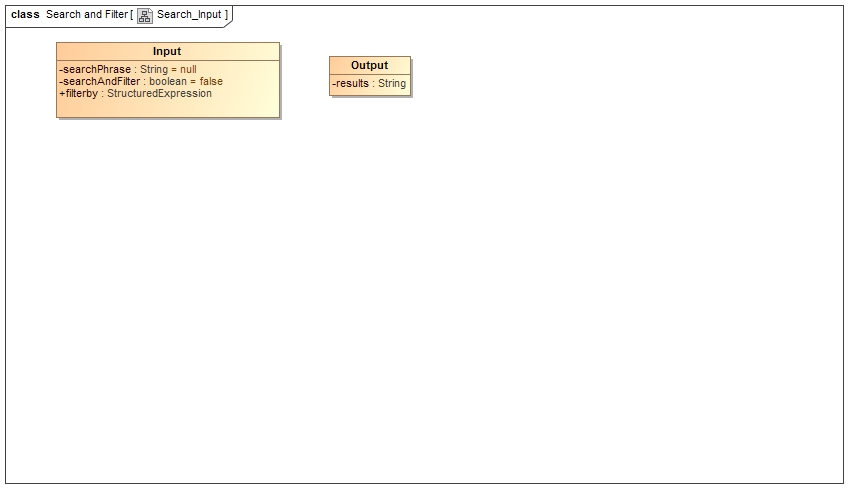
\includegraphics{Images/SearchAndFilter/Search_Input_output}
\\
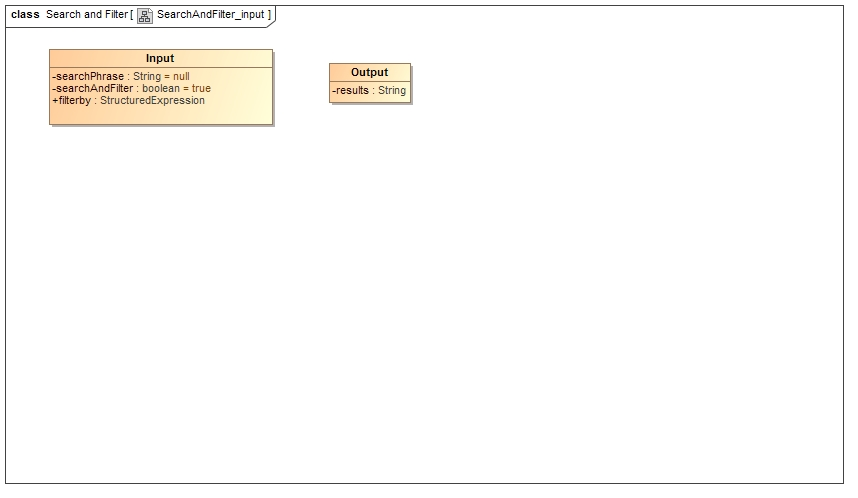
\includegraphics{Images/SearchAndFilter/SearchAndFilter_input_output}
\\
\\
\textbf{Required Functionality/Use case diagram}
\\
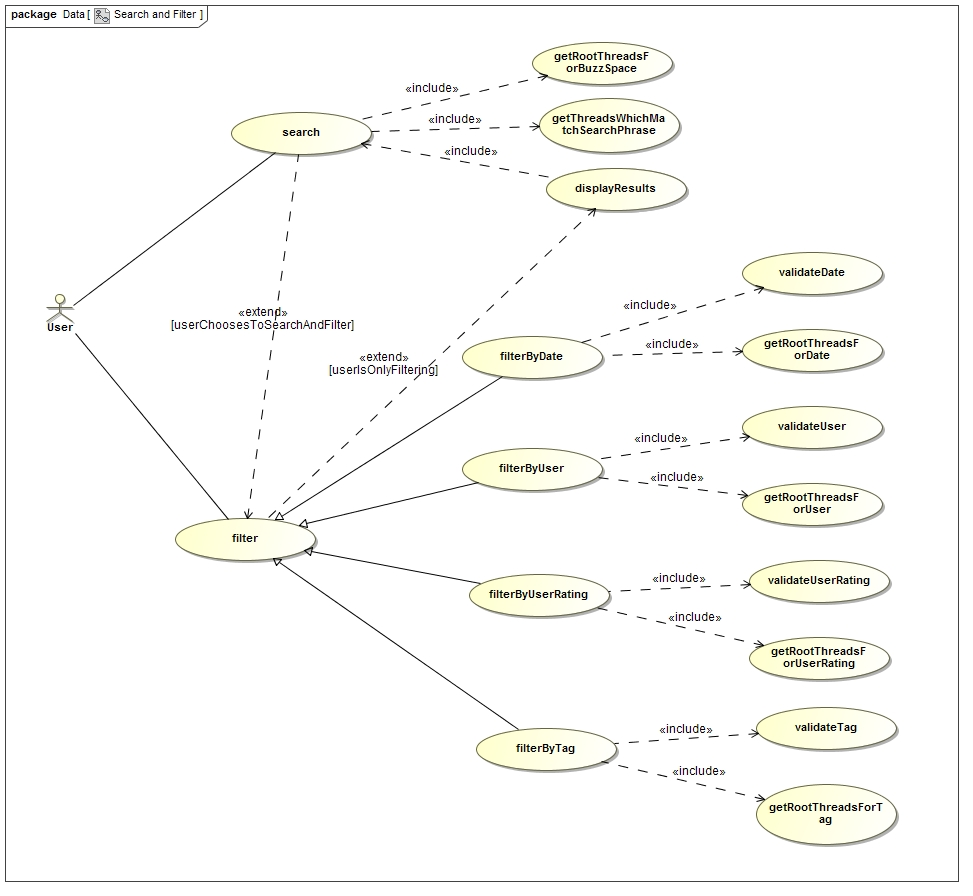
\includegraphics{Images/SearchAndFilter/SearchAndFilter_usecase}
\\
\\
\textbf{Process specifications}
\\
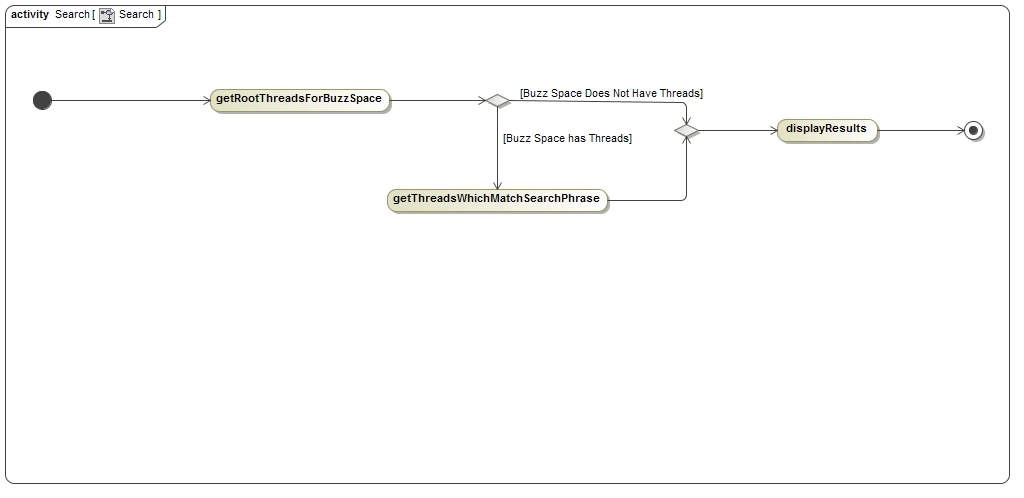
\includegraphics{Images/SearchAndFilter/Search_processSpecification}
\\
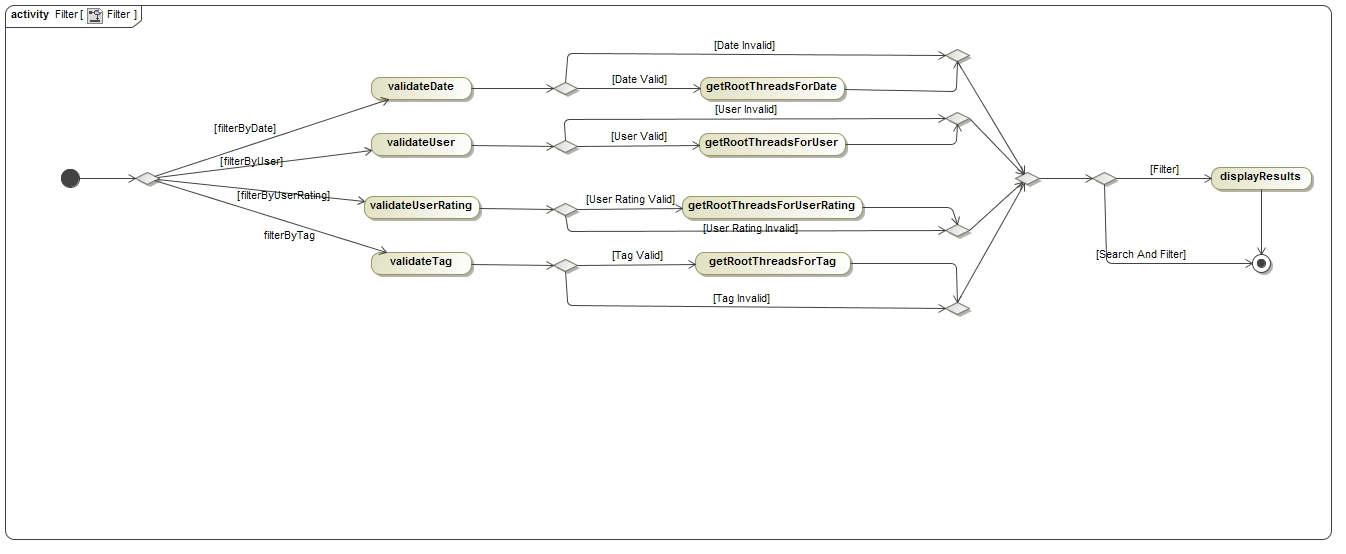
\includegraphics{Images/SearchAndFilter/Filter_processSpecification}
\\
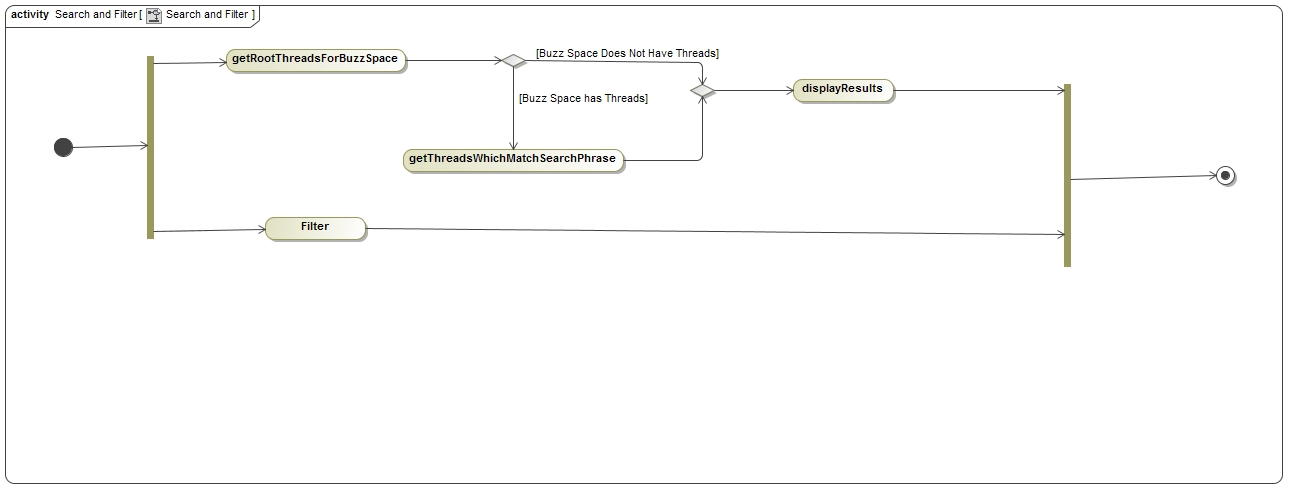
\includegraphics{Images/SearchAndFilter/SearchAndFilter_processSpecification}
\\
\\
=======
>>>>>>> origin/master

Prenolan
\subsubsection{Voting and Evaluation}
\textbf{Pre-Condition}: A post has to have been created for a user to be able to vote on or evaluate it. Any user can vote on or evaluate a post as long as the user is logged in and a part of a specific Buzz Space. An exception to this rule is when the administration of a Buzz Space set specific rules as to which users (perhaps based on status) can vote on or evaluate posts.
\\
\textbf{Post-Condition:} A vote or evaluation has to be visible to every user (or only some based on the administration of that space) after it has been made on a post. A positive vote or evaluation has to reflect upon the posters progress to the next status level.
\\
\\
\includegraphics{Images/VotesAndEvaluation/Class_Diagram__Input}
\includegraphics{Images/VotesAndEvaluation/Class_Diagram__Output}
\\
\subsubsection{Best Answer}
\textbf{Pre-Condition}: A user must have the privileges set by the administration of a space in order to mark a post as the best answer. The user is required to be logged in.
\\
\textbf{Post-Condition}: The thread should effectively display that an answer has been selected and optionally close the thread. The poster of the best answer should acquire an increase in progress to the next status level.
\\
\\
\includegraphics{Images/BestAnswer/Class_Diagram}
\\
\\
Lutfiyya\\
\subsubsection{Evaluation Report}
\textbf{Pre-Condition}: A lecturer has to be a registered user of a Buzz Space and must also be logged in to be able to generate an evaluation report of the students. The UserID of a participant should exist for reporting purposes.
\\
\textbf{Post-Condition:} A lecturer should get statistical information about each student and generate an evaluation report for a participant
\\
\\
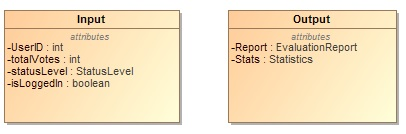
\includegraphics{Images/Report/Input&Output}
\\
\\
Maria\\

\subsection{Required functionality}
Jessica and Michelle\\
Jimmy\\
Ephi\\
\begin{center}
\includegraphics[width=0.9\linewidth]{./Images/ManageUserProfile/functional_requirements}
\end{center}
Thabang\\
Prenolan\\
\begin{center}
\includegraphics[width=0.9\linewidth]{./Images/VotesAndEvaluation/functional_requirements}
\end{center}

\begin{center}
\includegraphics[width=0.9\linewidth]{./Images/BestAnswer/functional_requirements}
\end{center}

Lutfiyya\\
\includegraphics[width=15cm,height=10cm]{./Images/Report/functional_requirements}\\
\\

Maria\\

\subsection{Process specification}
Jessica and Michelle\\
Jimmy\\
Ephi\\

\begin{center}
\includegraphics[width=0.9\linewidth]{./Images/ManageUserProfile/functional_requirements}
\end{center}

Thabang\\
Prenolan\\
\begin{center}
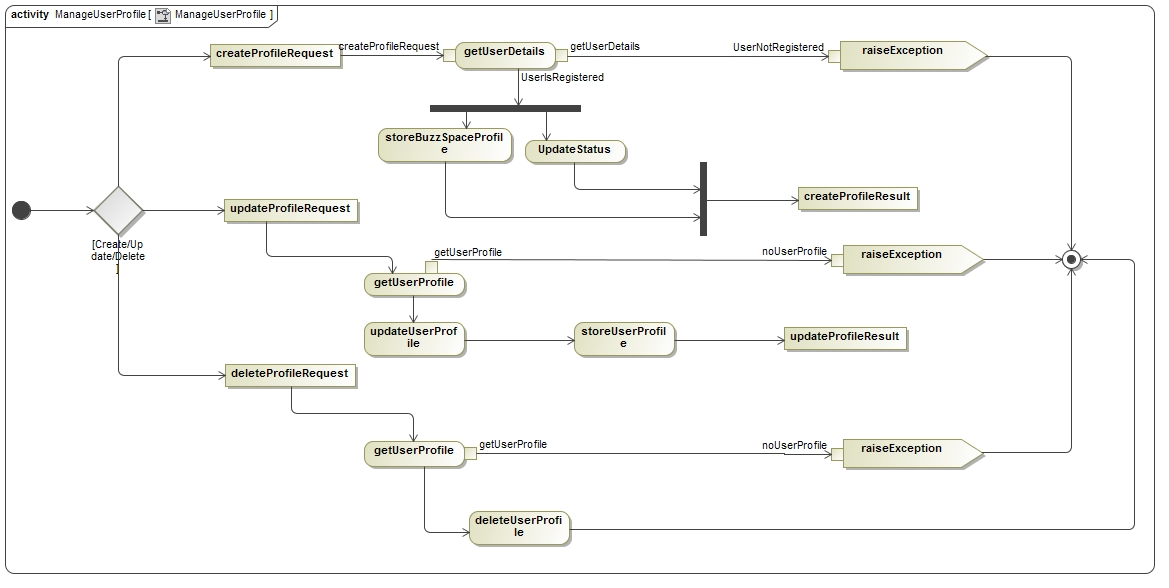
\includegraphics[width=0.9\linewidth]{./Images/VotesAndEvaluation/process_specification}
\end{center}

\begin{center}
\includegraphics[width=0.9\linewidth]{./Images/BestAnswer/process_spec}
\end{center}

Lutfiyya\\
%\begin{figure}
%\centering
\includegraphics[width=15cm,height=10cm]{./Images/Report/process_spec}
%\caption{Process specification for evaluation of reports}
%\end{figure}

Maria\\

\subsection{Domain model}


\end{document}

